% =============================================================================
% DIFERENÇA-EM-DIFERENÇAS (15:10 a 15:35)   [Script 04 | Exercício 2]
% =============================================================================
\section[DiD]{Diferença-em-diferenças}

\begin{frame}{A ideia: comparar variações}
  \begin{block}{Dupla diferença}
    \small
    $$\text{DD}=(\bar Y_{T}^{\,depois}-\bar Y_{T}^{\,antes})-(\bar Y_{C}^{\,depois}-\bar Y_{C}^{\,antes})$$
  \end{block}
  \begin{itemize}
    \item A variação do \textbf{controle} é a tendência que o tratado teria seguido sem a política;
    \item Elimina diferenças \emph{fixas} entre os grupos, mesmo as não observadas;
    \item Pressuposto central: \destaque{tendências paralelas}.
  \end{itemize}
\end{frame}

\begin{frame}{Exemplo numérico}
  \begin{columns}[T]
    \begin{column}{0.4\textwidth}
      \footnotesize
      \renewcommand{\arraystretch}{1.3}
      \begin{tabular}{lrr}
        \toprule
        \textbf{Renda} & \textbf{Part.} & \textbf{Não} \\ \midrule
        Antes & 80 & 90 \\
        Depois & 125 & 120 \\ \midrule
        Variação & +45 & +30 \\ \bottomrule
      \end{tabular}
      \vspace{0.3cm}

      DD $=45-30=$ \destaque{15}\\[4pt]
      {\scriptsize Antes-depois: 45 (superestima). Participantes $\times$ não: 5 (subestima).}
    \end{column}
    \begin{column}{0.6\textwidth}
      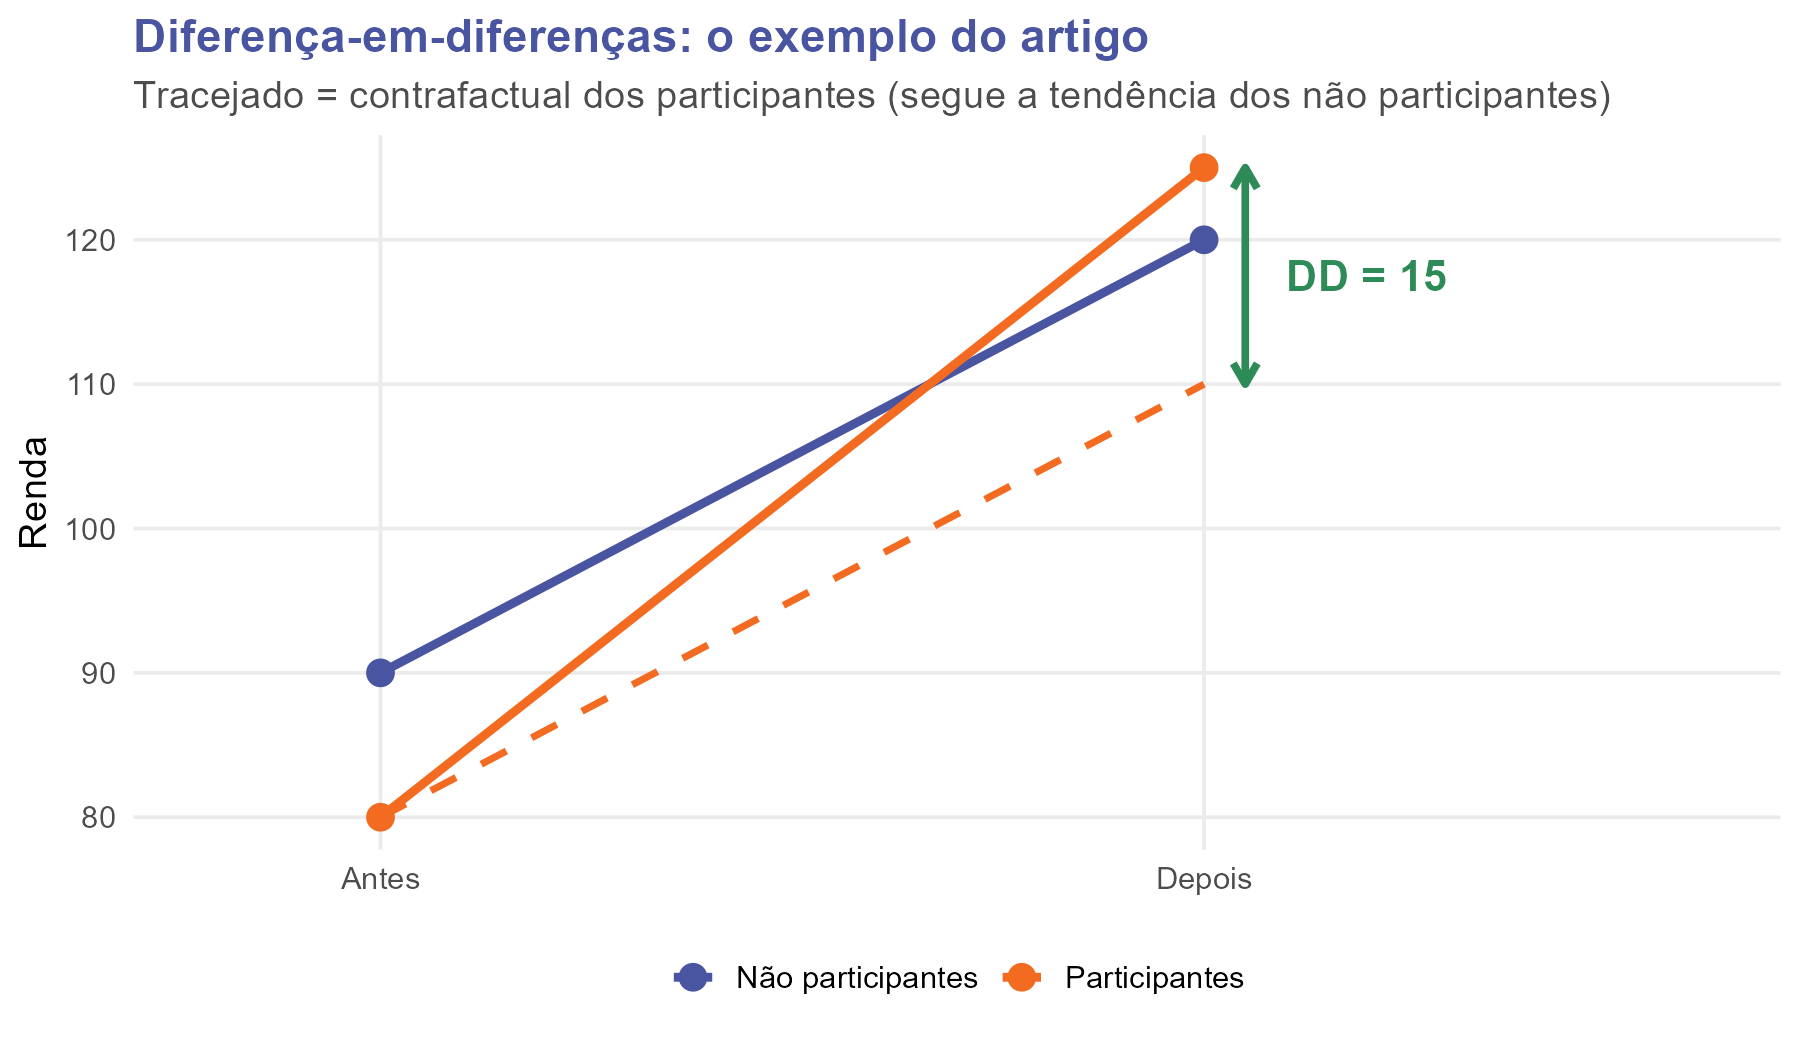
\includegraphics[width=\textwidth]{04_figura6.png}
    \end{column}
  \end{columns}
  \fonte{Exemplo adaptado de Khandker, Koolwal e Samad (2010).}
\end{frame}

\begin{frame}{Diferença-em-diferenças: características e exemplos}
  \carac{a \textbf{tendência do grupo de controle} aplicada ao tratado}
        {\textbf{tendências paralelas} na ausência da política; sem antecipação; sem contaminação}
        {efeito sobre os tratados (ATT)}
        {dados \textbf{antes e depois} de tratados e controles (painel ou cortes repetidos)}
        {política implantada só em parte do território ou da população; leis}
  \vspace{0.15cm}
  \textbf{\footnotesize\color{azul}Exemplos em políticas públicas}\par
    \scriptsize
    \begin{itemize}
      \item \textbf{Brasil:} Lei Maria da Penha. Mulheres (tratamento) $\times$ homens (controle), taxa de homicídios (Cerqueira et al., 2015).
      \item \textbf{EUA:} aumento do salário mínimo em Nova Jersey, com lanchonetes da Pensilvânia como controle (Card e Krueger, 1994).
      \item \textbf{Hipotético:} bolsa-permanência em algumas escolas (Exercício 2); Qualifica numa região (script 04).
    \end{itemize}
  
\end{frame}

\begin{frame}{Simulação: tendências paralelas antes do programa}
  \centering
  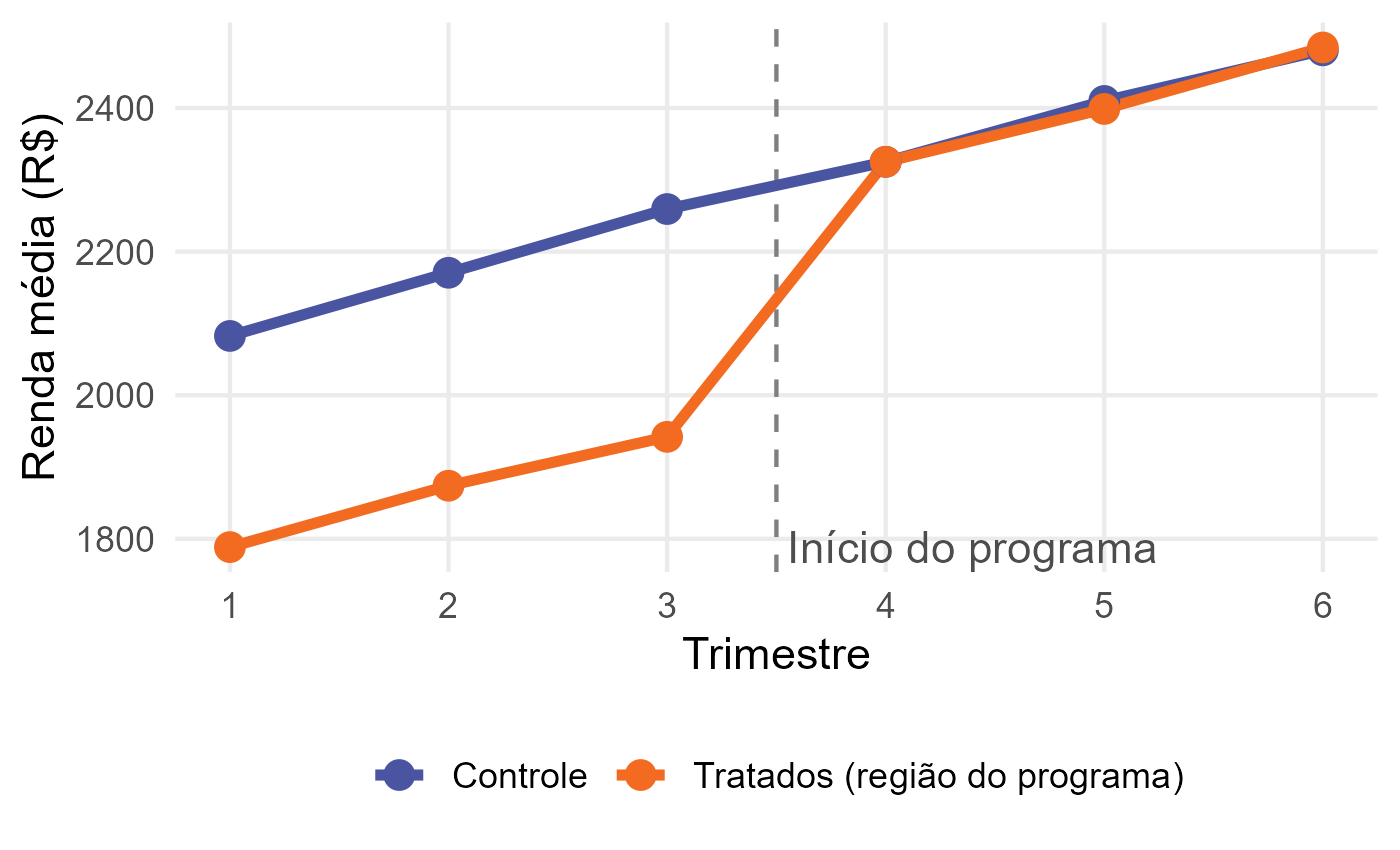
\includegraphics[height=3.9cm]{04_tendencias.png}\par
  \footnotesize Os tratados partem de um nível menor (mais pobres), mas \textbf{evoluem em paralelo} até o 4.º trimestre, quando começa o programa.
\end{frame}

\begin{frame}{Passo a passo: diferença-em-diferenças (1 de 2)}
  \relax{\scriptsize\setlength{\tabcolsep}{2.5pt}\renewcommand{\arraystretch}{1.1}\begin{tabular}{@{}cP{2.55cm}P{2.75cm}P{3.6cm}@{}}
    \toprule
    \cabecalho{Como ler e decidir}
    \linha{1}{Olhe as tendências \textbf{antes} da política}{tratados: 1.789; 1.874; 1.942\newline controle: 2.083; 2.171; 2.259}{Sobem ${\approx}$ +80 por trimestre nos dois: \textbf{paralelas}.}
    \linha{2}{Calcule as \textbf{4 médias} (antes/depois, tratado/controle)}{tratados: 1.868 $\to$ 2.403 (+534)\newline controle: 2.171 $\to$ 2.405 (+234)}{Os dois sobem. A variação do controle (+234) é a tendência.}
    \ultimalinha{3}{\textbf{Dupla diferença}}{DD = 534 $-$ 234 = 300}{O programa elevou a renda em R\$ 300 \textbf{além da tendência}. (Antes-depois: 534.)}
  \end{tabular}}
\end{frame}

\begin{frame}{Passo a passo: diferença-em-diferenças (2 de 2)}
  \relax{\scriptsize\setlength{\tabcolsep}{2.5pt}\renewcommand{\arraystretch}{1.1}\begin{tabular}{@{}cP{2.55cm}P{2.75cm}P{3.6cm}@{}}
    \toprule
    \cabecalho{Como ler e decidir}
    \linha{4}{Regressão com \textbf{interação} e erro-padrão por \emph{cluster}}{tratado:pos = 300,2\newline EP = 7,8\newline IC 95\%: 285 a 315}{Mesmo número do passo 3, agora com incerteza.}
    \linha{5}{\textbf{Estudo de eventos}: efeito por trimestre (ref.: 3.º)}{antes: +23 e +21 (EP 34)\newline depois: 317, 306, 321}{Antes ${\approx}$ 0 (sem pré-tendência). Depois ${\approx}$ 300, estável.}
    \ultimalinha{6}{\textbf{Placebo}: finja o programa mais cedo}{DD placebo = $-13$}{Perto de zero: ok. Se fosse grande (no cenário ruim: +47), \textbf{desconfie}.}
  \end{tabular}}
  \caixaconclusao{DD = R\$ 300 (verdade: 300), com tendências paralelas confirmadas por dois testes.}
\end{frame}

\begin{frame}{Quando as tendências \textit{não} são paralelas}
  \centering
  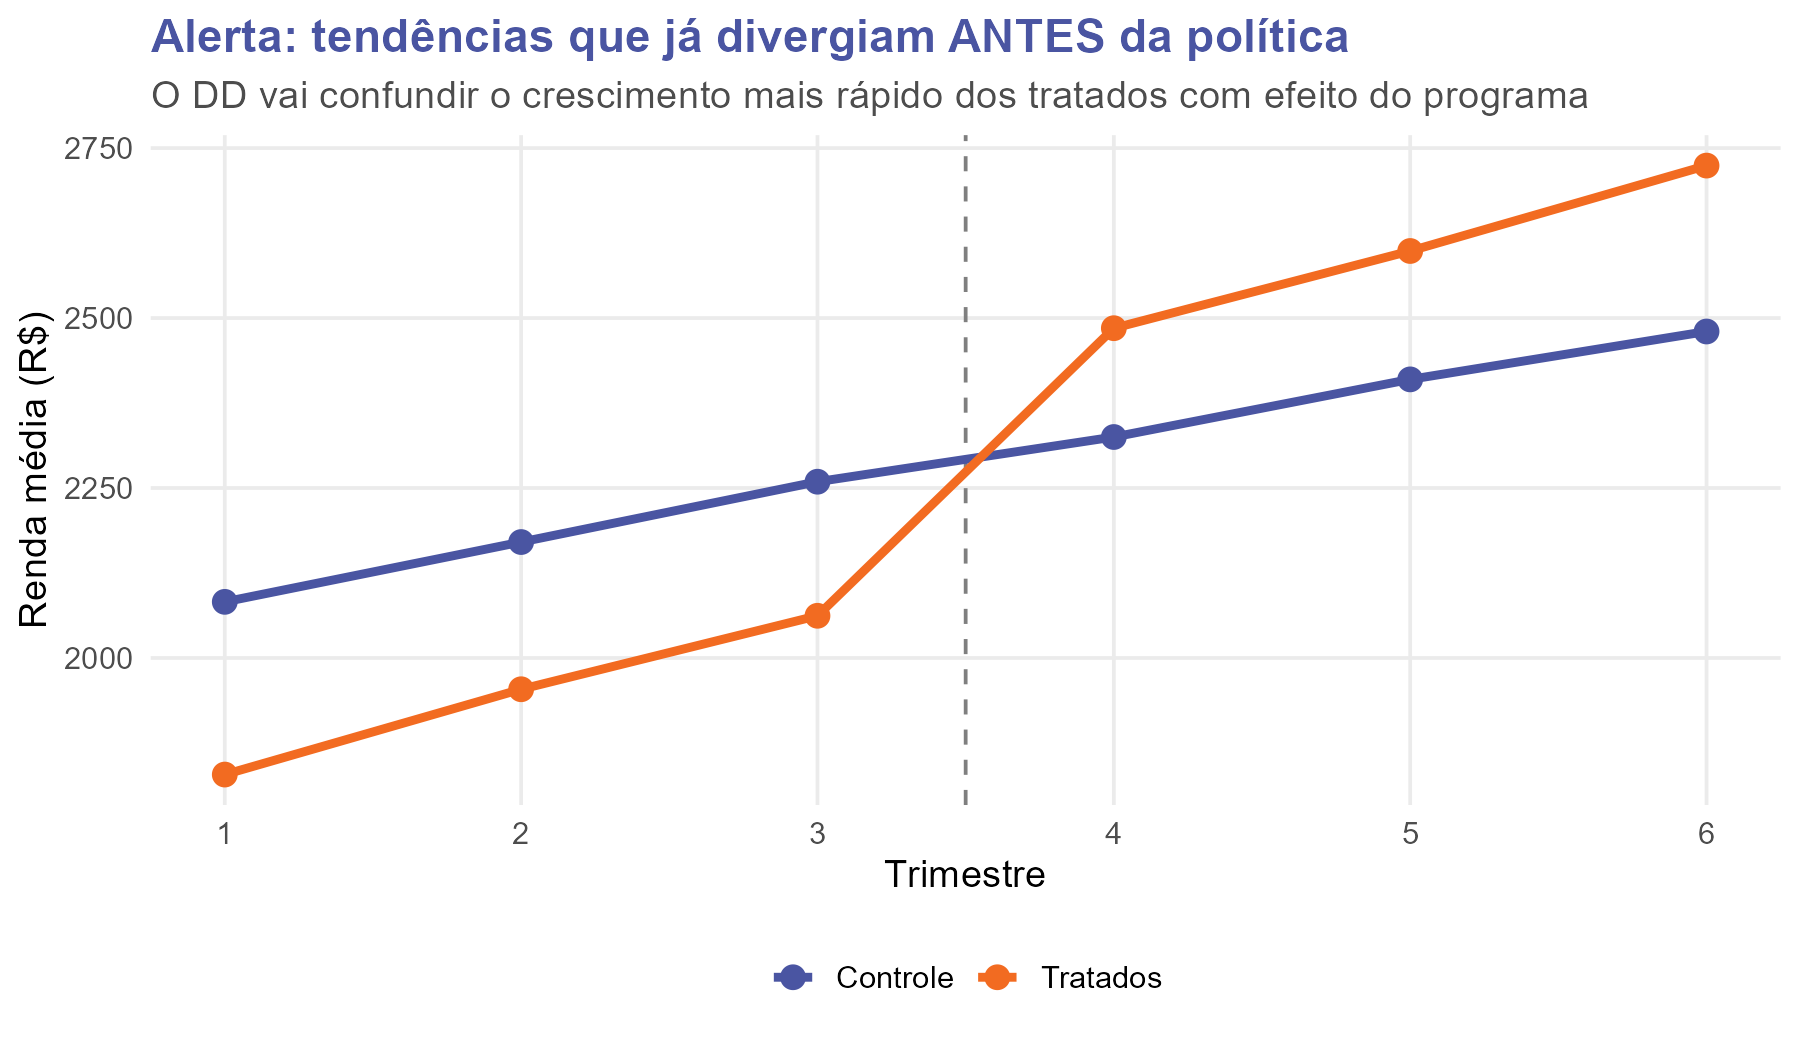
\includegraphics[height=4.0cm]{04_nao_paralelas.png}\par
  \footnotesize Os tratados já cresciam mais rápido: o DD estima \alert{R\$ 420} (verdade: 300). O \textbf{placebo} denuncia o problema: +47.
\end{frame}

\begin{frame}{Exercício 2: diferença-em-diferenças (10 min)}
  \begin{exerciciobox}{\texttt{atividades/exercicio\_02\_diferenca\_em\_diferenca.R}}
    \small
    \begin{enumerate}
      \item Calcule o DD de uma bolsa-permanência (evasão de 12\% para 8\% nas escolas com programa; de 10\% para 9\% nas demais);
      \item Gere um painel com tendência extra de R\$ 20/trimestre para os tratados: o DD acerta? O placebo avisa?
    \end{enumerate}
  \end{exerciciobox}
  \vspace{0.2cm}
  \textbf{Para pensar (Lei Maria da Penha):} que evento poderia afetar mulheres e homens de forma diferente e violar as tendências paralelas?
\end{frame}
